\vspace*{-1.5cm}
\chapter{Results}

We consider satellite altitudes of 500 km up to 10,000 km, incrementing by 500 km. In terms of ground station (gs) separation, \(d\), we consider values from 500 km, roughly the distance from Zacatecas, Zac., MX to Ciudad de M\'{e}xico, to 2,000 km, roughly the distance from Zacatecas, Zac., MX to the Los Angeles, CA. \(d\) is also incremented by 500 km. We implement a Bernoulli process in our simulations and give the satellite a total of 500 orbits for each configuration. The following presentation is that of the averages of our simulation data.

\section{Success Rate}

A success is when the satellite is able to link with both ground stations. Once a success occurs, we store the time at which it occurred as well as the first link age. The satellite then `dumps' the success and attempts to generate another one. Fig. \ref{fig:success-counts} shows the number of successes the satellite is able to achieve per orbit as a function of \(h\) for different values of \(d\). The \textcolor{mygreen}{green} curve shows the trend one would expect: less successes are produced as the satellite altitude increases. The \textcolor{mypurple}{purple} and \textcolor{myred}{red} curves, however, tell a different story. These curves tell us that there exists an optimal value of \(h > \min\qty{h}\) at which the success counts are maxmized. In both cases, this optimal value is \(h = 1,000\) km. Interstingly we also notice that the gs separation becomes irrelevant for large values of \(h\).

\begin{wrapfigure}[19]{r}{0.5\textwidth}
    \centering
    \vspace{-.1\baselineskip}
    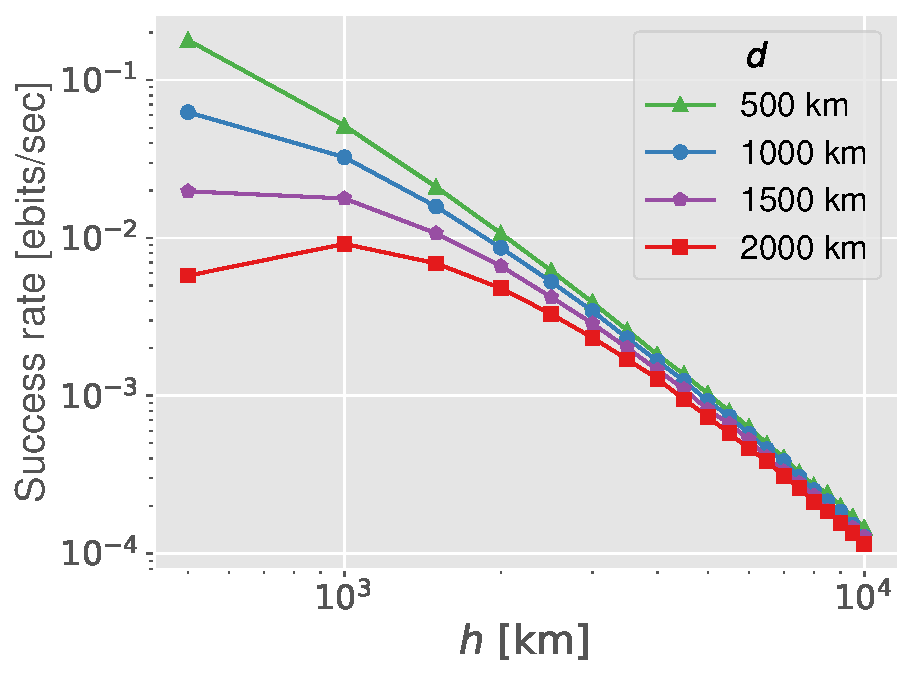
\includegraphics[width=0.5\textwidth]{figures/success-rate.pdf}
    \caption{}
    \label{fig:success-rate}
\end{wrapfigure}

A success rate is shown in Fig. \ref{fig:success-rate}. This rate is computed by the quotient of the number of ebits per orbit (seen in Fig. \ref{fig:success-counts}), divided by the amount of time the satellite spends in visibility:
\begin{equation}
    T_{\text{vis}} = \frac{\theta^f - \theta^0}{\omega_\theta - \omega_e},
\end{equation}
where
\begin{equation*}
    \theta^f \equiv \pi - \theta^0.
\end{equation*}
We divide by this visibility time rather than the period of the orbit since \(T_{\text{vis}} = T_{\text{vis}} \qty(h, d)\) while the the typical period is only a function of \(h\).

We notice that the rates produced in Fig. \ref{fig:success-rate} are much smaller than that in \cite{khatri2021}. This is due to the fact that we have only one ground station our satellite lacks the ability to simultaneously communicate with both gs. Computing the inverse of the data in Fig. \ref{fig:success-rate} thus gives us the expected waiting time for a success. Note, by definition, this is the average amount of time it would take to generate the second link conditioned on the first link already being generated.

\begin{wrapfigure}[14]{l}{0.5\textwidth}
    \centering
    \vspace{-.1\baselineskip}
    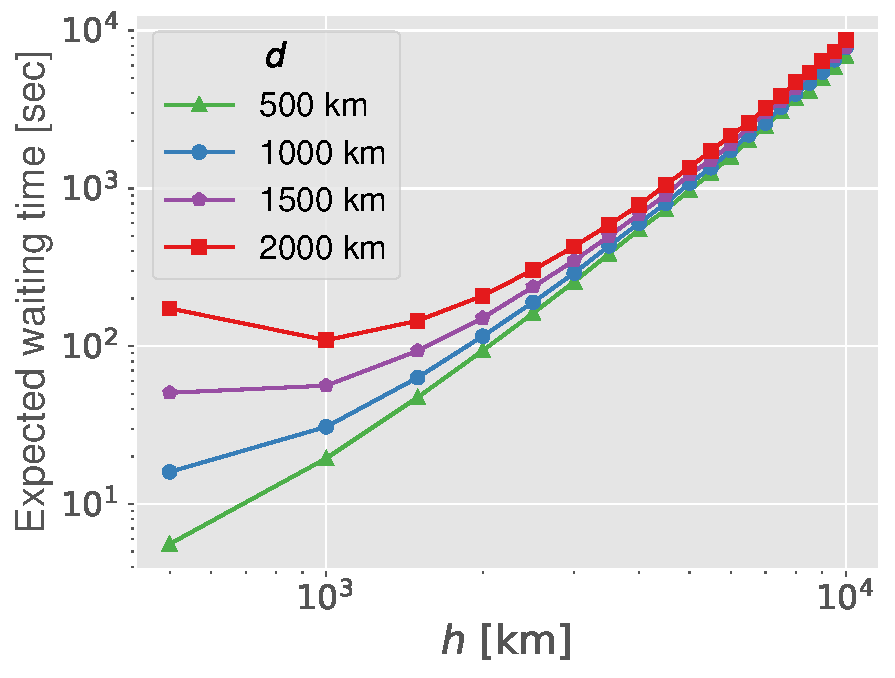
\includegraphics[width=0.5\textwidth]{figures/exp-time.pdf}
    \caption{}
    \label{fig:exp-time}
\end{wrapfigure}

Fig. \ref{fig:exp-time} shows that the minimum expected waiting time is 5.6 sec and occurs for a gs separation of 500 km and a satellite altitude of the same value. The largest expected waiting time occurs for \(h =\) 10,000 km, \(d =\) 2,000 km, with a value of 2.4 hrs. At this same altitude, the smallest value of \(d\) produces an expected waiting time of 1.9 hrs. Keeping these times in mind, in the following section we explore the values that the simulation actually produced.

\section{First Link Age}

Given that the first ground station has succesfully been linked, the first link age is the amount of time it took to generate a succesful link with the second ground station. Since we assume decoherence occurs only on gs memory, this figure of merit is the direct channel to studying how quantum information is affected in a system like the one we are considering.

Fig. \ref{fig:exp-time} told us that satellite altitude is relevant when it comes to expected waiting time, or what we will now call first link age, unlike the behavior we saw in Fig. \ref{fig:success-counts}. The actual data produced by the simulations goes against this and aligns with Fig. \ref{fig:success-counts}. In Fig. \ref{fig:fla}, we see that, starting at \(h =\) 4,000 km (black, dashed line), the first link age is identical for all configurations. We also see, from the \textcolor{myred}{red} and \textcolor{mypurple}{purple} curves in Fig. \ref{fig:fla}, larger values of \(d\) do not necessarily benefit from the smallest value of \(h\). Like in \ref{fig:success-counts}, the best outcome for these curves arrives from a satellite altitude of \(h = 1000\) km. Also, while Fig \ref{fig:exp-time} predicts a minimum first link age of 5.6 sec, Fig \ref{fig:fla} reveals that the actual minimum is 0.42 sec; 7.6\% of the expected value!

\begin{wrapfigure}[16]{r}{0.5\textwidth}
    \centering
    \vspace{-.1\baselineskip}
    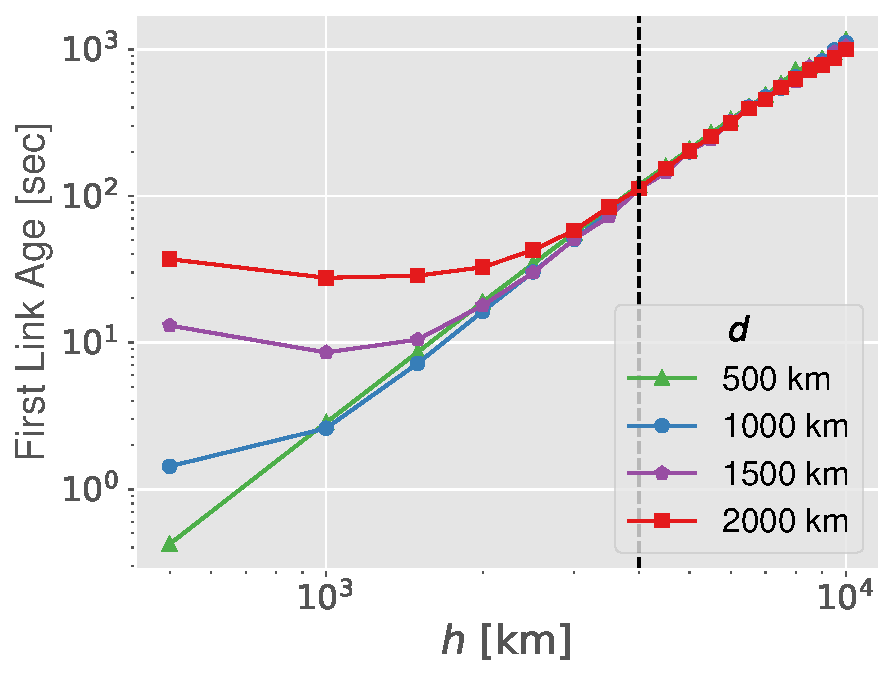
\includegraphics[width=0.5\textwidth]{figures/fla.pdf}
    \caption{}
    \label{fig:fla}
\end{wrapfigure}

Additionally, the largest first age occurs for \(d =\) 500 km\footnote{One would naturally anticipate that the smallest value of \(d\) would always produce the best first link age. However, we've found that for \(h >\) 8,000 km the behavior flips and the smallest first link age is produced by the largest value of \(d\). However, the `best' first link is only \(\sim\)90\% of the worst one in those regions so we don't make a huge point at this difference. Larger values of \(h\) and more values of \(d\) must be considered to confidently establish a trend.} and \(h =\) 10,000 km, with a value of 0.32 hrs. This is 13\% of the value extracted from Fig. \ref{fig:exp-time}.

\section{Quantifying Entanglement}

As a bridge to material we learned in the second half of the class, we take the data in Fig \ref{fig:fla} and see how we can quantify the resulting entanglement between the two gs. We consider two metrics: fidelity and entanglement of formation \cite{wootters1998}. Concretely, we assume the shared Bell state is \(\ket{\Phi^+}\), we apply the single-qubit depolarizing channel to the qubit that is stored on the first gs while the satellite attemps to link with the second one. We assume Markovian \cite{brand2024} noise, where the depolarization rate is \(\gamma = 0.01\) (to counteract the large values we have for the first link age). Under these \textit{super realistic} conditions, we are able to generate Fig. \ref{fig:quant}.

\begin{figure}[h]
    \centering
    \begin{subfigure}[b]{0.4\textwidth}
        \centering
        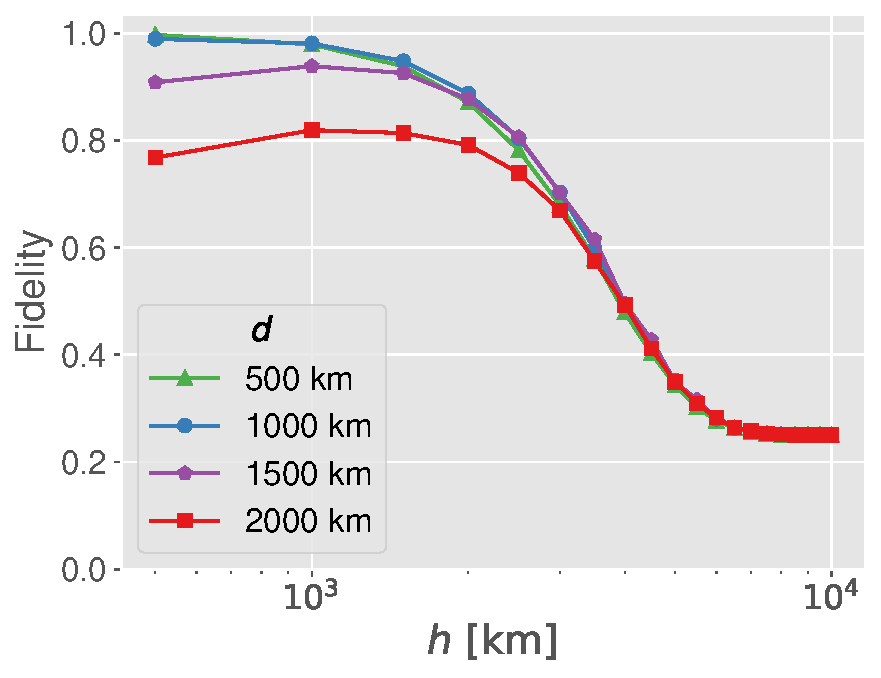
\includegraphics[width=\textwidth]{figures/fidelity.pdf}
        \caption{}
        \label{fig:fid}
    \end{subfigure}
    \hspace{1cm}
    \begin{subfigure}[b]{0.4\textwidth}
        \centering
        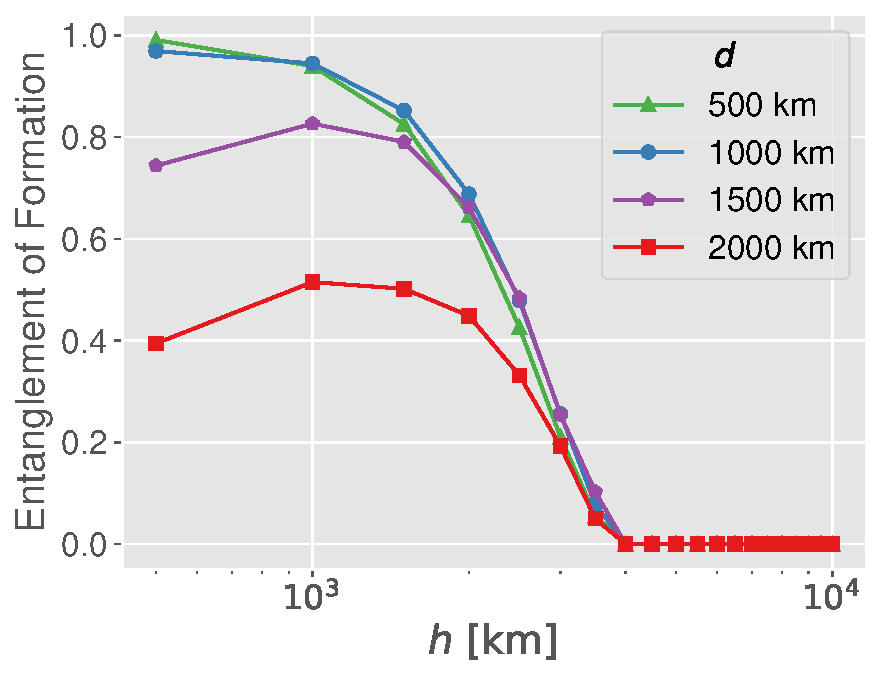
\includegraphics[width=\textwidth]{figures/eof.pdf}
        \caption{}
        \label{fig:eof}
    \end{subfigure}
    \caption{}
    \label{fig:quant}
\end{figure}

\vspace*{-0.5cm}
\section{Conclusions}

My favorite thing I learned in this course is that ``\textbf{fidelity can be a misleading measure of quantum entangled state quality}'' \cite{vardoyan2025}. I have kept it in mind throughout this project and in my own research. The investigation performed here often went against intuition. It is unexpected that the lowest satellite altitude is not always optimal. It is also not expected that a difference in gs spacing of 500 km produces the same fidelity and entanglement of formation, as seen in Fig. \ref{fig:quant}. Fig. \ref{fig:quant} shows similar trend between fidelity and entanglement of formation when it comes to the vairances in \(h\) and \(d\). However, we see that the entanglement of formation values do eventually hit zero while the fidelity never does.

Nevertheless, in this simple experiment we are able to show that satellite communication rates \textit{can} be great, even at an altitude of 500 km. We've skewed the depolariation rate to give us nice-looking figures but further investigation into optimal satellite placement can produce results comparable to what we have here with more realistic values.